
\chapter{Analysis and High-Level Design}

It is the goal of this thesis to enable detection of sleep-related illnesses 
with the aid of an Android device and low-cost sensors, and to further analyze 
and evaluate sleep- and breath-related patterns. We developed an application, 
called \textit{Nidra}, which attempts to collect, analyze and share data collected 
from external sensors, all on a mobile device. Also, Nidra acts as a platform for 
modules to enrich the data, thus extending the functionality of the application.

The motivation behind this application is to provide an interface for patients 
to potentially run a self-diagnostic (of the illness?) from home, and to aid 
researchers and doctors with analysis of sleep- and breathing-related illnesses 
(e.g., Obstructive Sleep Apnea). An overview of the Nidra application pipeline 
can be found in figure x, beginning with data acquired from a sensor, and ending 
with the data in the Nidra application. As for now, Nidra consists of three 
main functionalities, each related to the requirements defined in Section [Problem Statement]. 

\begin{enumerate}
    \item The application should provide an interface for the patient to 1) record physiological signals (i.e., during sleep); 2) present the results; and 3) export/import the results.
    \item The application should provide an interface for the developers to create modules to enrich the data from records or extend the functionality of the application. 
    \item The application should ensure a seamless and continuous data stream, uninterrupted from sensor disconnections and human disruptions.
\end{enumerate}

This chapter will give a detailed look at the design of Nidra...

\section{High-Level Design}

\subsection{Stakeholders}
A stakeholder is a term coined to describe those persons or organizations that have, or claim an interest in the project. Identifying stakeholders is essential to fulfilling the requirement set in the thesis, as they contribute to form and sculpture the application. As discussed by McGrath \textit{et al}. \cite{stakeholderdefined}, stakeholders can be distinguish  into four categories: 1) \textit{contributing (primary) stakeholders} are those that participate in developing and sustaining the project; 2) \textit{observer (secondary) stakeholder} are those who affect or influence the project;  3) \textit{end-user (tertiary stakeholder)} is the one who interact and uses the output of the application; and 4) \textit{invested stakeholder} is one who has control of the project. In Nidra, we have three stakeholders who affect the application, and each can be categorized respectfully.
\begin{itemize}
    \item \textbf{Patients} - are identified as an end-user; they interact with the application.  
    \item \textbf{Researchers/Doctors} - are identified as an observer stakeholder; they might not use the application itself. However, they might use the data obtained from the patients' recordings for further analysis. Additionally, request functionality in the application.
    \item \textbf{Developers} - are identified as a contributor stakeholder; they maintain the application from bugs or extend the functionally of the application. Additionally, they can contribute to developing modules that extend the functionality of the application. 
\end{itemize}

\subsection{Task Analysis}
Task analysis is a methodology to facilitate the design of complex systems. Hierarchical task analysis (HTA) is an underlying technique that analyzes and decomposes complex tasks such as planning, diagnosis, and decision making, into specific subtasks [Task analysis...]. In this Section, we will be analyzing system tasks and user-related tasks.

%\subsubsection{System Tasks}

\noindent\textbf{Recording}

\noindent A \textit{recording} is a process of collecting and storing physiological signals (e.g., breathing data) from sensors over an extended period (e.g., overnight). To enable a recording, we need to establish connections to available sensors, collect samples from the sensors, and store the samples on the device. A \textit{sensor} is a device that transforms analog signals from the real world into digital signals. The digital signals are transmittable over Link Layer technologies (e.g., BlueTooth), and the communication between a sensor and device occurs based on the protocols the sensor supports. A \textit{sample} is a single sensor reading containing data and metadata, such as time and the physiological data. During the recording session, ensuring that the sensors and the devices maintain connectivity such that the record contains meaningful data.  Once a recording session has terminated, a \textit{record} with metadata about the recording session is stored, alongside the samples.    

\noindent \textbf{Sharing}

\noindent Sharing is a mechanism to export and import records across applications. \textit{Exporting} consists of bundling one or more records with correlated samples into a transmittable format and transferring the bundled records over a media (e.g., mail). \textit{Importing}, on the other hand, consists of locating the bundled records on the device, parsing the content and storing it on the device. The sharing mechanism allows the patients to send their records to researchers/doctors.

\noindent \textbf{Module}

\noindent A \textit{module} is an independent application that is installed and launched in Nidra (hereafter: application), to provide extended functionality and data enrichment. A module does not necessarily interact with the application. However, it utilizes the data (e.g., records). For example, a module could be using the records to feed a machine-learning algorithm to predict obstructive sleep apnea. Installing a module is achieved by locating the module-application on the device, and storing the reference in the application. Due to limitations in Android, the module-application cannot be executed within the application. Therefore, the module-application is a standalone Android application. Furthermore, the development of the module-application is independent of the application. 

\noindent \textbf{Analytics}

\noindent Analytics is the visualization and interpretation of patterns in the records. The application facilitates the recording of breathing data, which enables the detection and analysis of sleep-related breathing disorder. There are various analytical methods, ranging from graphs to advanced machine learning algorithms, and incorporating a simple time series plot can indirectly aid in the analysis. For example, plotting a time series graph where the breathing data are on the Y-axis and the time on X-axis, provides a graphical representation of the data that can be further analyzed within the application.

\noindent \textbf{Storage}

\noindent Storage is the objective of achieving persistent data; data remain available after application termination. To enable storage, we use a database for a collection of related data that is easily accessed, managed, and updated. The database should be able to store records, samples, modules, and biometrical data related to the user (i.e., gender, age, height, and weight). Structuring a database that is reliable, efficient, and secure is a crucial part of achieving persistent storage. Android provides several options to enable storage on the device (e.g., internal storage and database).

\noindent \textbf{Presentation}

\noindent Presentation is the concept of exhibiting the functionality of the application to the user. A user interface (UI) is the part of the system that facilitates interaction between the user and the system. In Nidra, determining the screen layout, color palette, interactions, and feedback on actions is part of the development of a user interface. 

\section{Seperation of Concerns}

\subsection{Recording}
There are several approaches to assemble components to achieve a recording, and we review an alternative structure. In Figure \ref{fig:hta_recording} we have an HTA graph, which illustrate the building blocks to enable a recording and their dependencies:

\begin{figure}
    \centering
    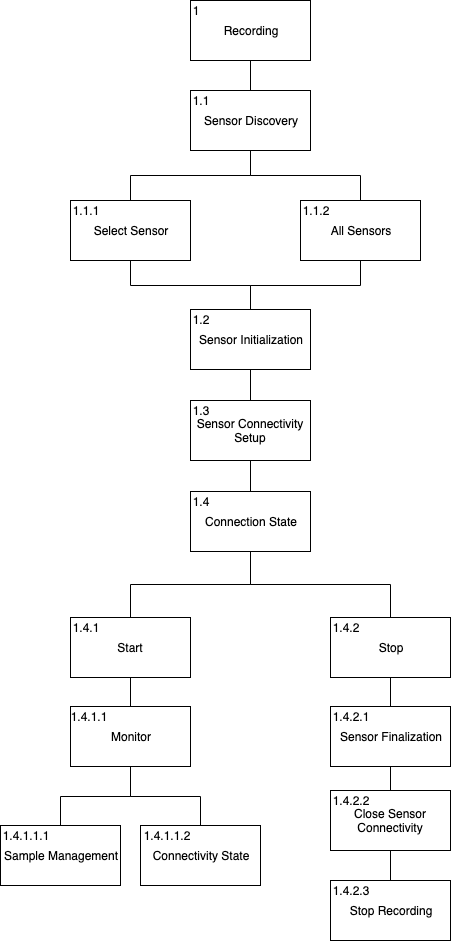
\includegraphics[width=0.65\textwidth]{images/Recording.png}
    \caption{Recording}
    \label{fig:hta_recording}
\end{figure}

\begin{itemize}
    \item Sensor Discover: Has to find all eligible sensors that can enable a recording.
    \item Select Sensors: From the sensor discovery, we can choose preferable sensors sources.
    \item  All Sensors: More straightforward, we sample from all of the available sensors.
    \item Sensor Initialization: Once we have a list of sensors sources, we need to establish and initialize a connection with the sensors. Occasionally a sensor might use some time to connect, or unforeseen occurrence is hindering the initialization of the sensor. Thus, blocking the state of the recording. 
    \item Sensor Connectivity Setup: Additionally, we establish a connection between the application and the sensor source. All data exchange occurs over the established interface. 
    \item Connection Stat: Based on sensors establishments we can proceed to either start or stop a recording. 
    \item Start: By starting, we notify the sensors to begin collecting data, and the view should display that a recording has begun accordingly.
    \item Monitor: Is continuously waiting for new samples to arrive on the interface defined between the application and the sensors.
    \item Sample Management: Once a new sample has arrived, we need to store the sample on a persistent storage.
    \item Connectivity State: If it is an external sensor, the sensor source might disconnect during a recording. Thus, implementing a mechanism to check for continuous data stream is a critical task.
    \item Stop: By stopping, we notify the sensors to stop collecting data from the sensor source.
    \item Sensor Finalization: We notify the sensor to stop sampling data, and close establishment.
    \item Close Sensor Connectivity: We close the interface establishment between the application and the sensors. 
    \item Stop Recording: Once the sensors has closed its connections, we can add additional information to the recording (e.g., title, description, rating). In the end, the recording has concluded and its stored on the mobile device.

\end{itemize}

This suggested structure of a recording is one alternative to enable a recording. Most of the components suggested in the structure are essential to a recording. A naive solution would be to ignore the connectivity state component, by assuming the sensors are connected indefinitely. In our thesis, we will be following 


\subsection{Sharing}

\subsection{Modules}

\subsection{Storage}

\subsection{Presentation}
